The application is the database entry point, and it is projected to be run either by a a government employee or a generic user. The starting page shows the two possible ways to access it.
\begin{figure}[h]
    \centering
    \begin{minipage}{0.475\textwidth}
        \centering
        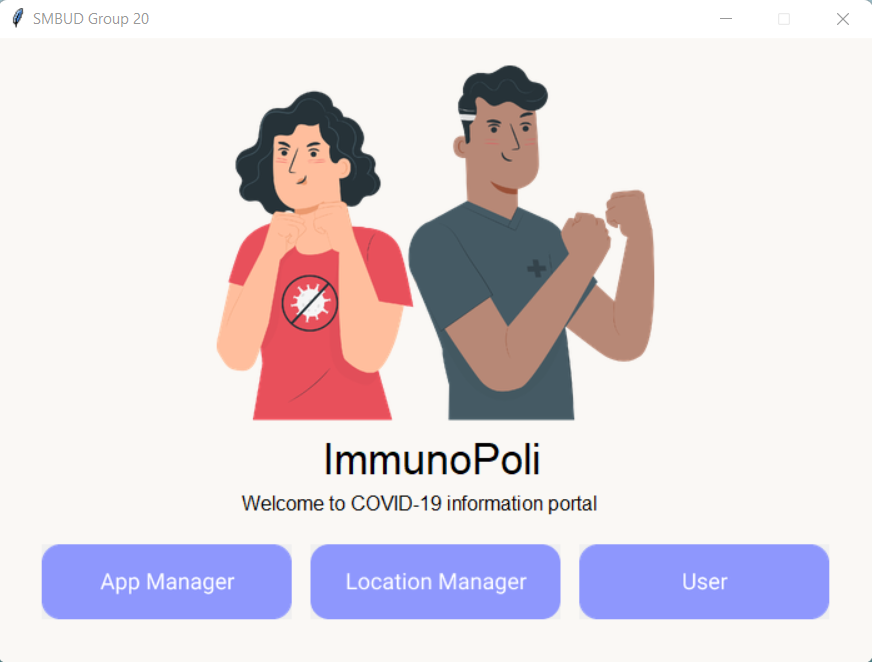
\includegraphics[width=\textwidth]{images/starting_page.png} 
        \caption{\textit{starting page}}
        \label{figure 2}
    \end{minipage}\hfill
    \begin{minipage}{0.475\textwidth}
        \centering
        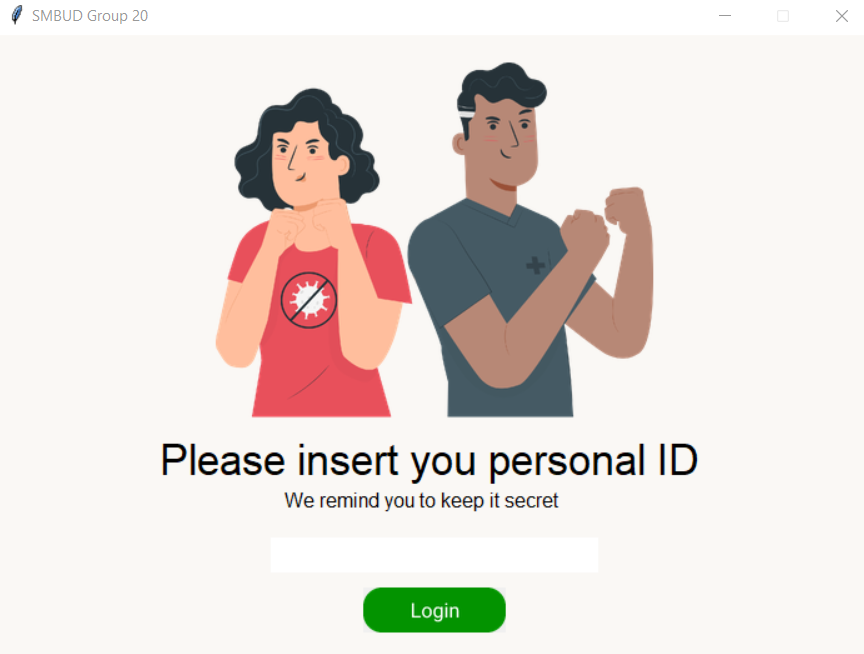
\includegraphics[width=\textwidth]{images/login_page.png} 
        \caption{\textit{login page}}
        \label{figure 3}
    \end{minipage}
\end{figure}
\newline
The first category of users has access to two features:
\begin{itemize}
    \item changing his/her personal information;
    \item examining the places he has visited and the risk he linked to them;
    \item checking his covid exposures;
    \item seeing the history of his tests and related outcomes.
\end{itemize}
The second category instead, has full access to the features:
\begin{itemize}
    \item adding information concerning COVID tests;
    \item monitoring COVID trends;
\end{itemize}
